\chapter{Aromatic Rings, Medicines, and Dyes}

\begin{kaichang}
Find a white tablet in your medicine cabinet, perhaps the common fever reducer acetaminophen, also called paracetamol. Then find blue jeans or a brightly colored T-shirt.

One swallowed, one worn: apparently unrelated. Yet enlarge their key molecules hundreds of millions of times, and the same component appears: a flat six-carbon hexagonal ring. The medicine uses it to hold its shape and fit protein crevices; dye uses it and linked similar structures to steal some colors from sunlight.

Guess what makes this hexagon so special that drugs and dyes both want it. By the end you should answer, and expose a misconception even textbook drawings can encourage.
\end{kaichang}

\section{Treasures from Coal Tar}

Begin with nineteenth-century town gas. London and Berlin streetlights burned gas from coal's destructive distillation, leaving unwanted black, sticky, pungent coal tar in factory corners. Chemists, however, liked rubbish heaps. In 1825, Faraday isolated a colorless liquid from lighting-gas condensate. Later found abundantly in coal tar, it proved to contain six carbons and six hydrogens per molecule.

This was benzene. It burned brightly but smokily, black smoke indicating an unusually high carbon fraction. Chapter 39's six-carbon hexane has fourteen hydrogens; benzene only six. So few hydrogens imply many extra carbon handshakes, high unsaturation in Chapter 36's terms.

Strangely, similarly unsaturated alkenes quickly decolorize reddish-brown bromine water by double-bond addition (Chapter 38), but benzene coexists with it almost unchanged. Alkene-like hydrogen deficiency, alkane-like steadiness: this tormented chemists for decades. Other strongly scented coal-tar liquids, pleasant to some noses and pungent to others, joined benzene under the romantic name \textbf{aromatic compounds}. Today aromatic has nothing to do with smell, but denotes structures typified by benzene. Remember: benzene itself is highly toxic, damages blood-forming tissues with prolonged inhalation, and is a proven human carcinogen. Aromatic never means pleasant and safe. All solvents in this section are teacher-demonstration or video only.

\section{Zoom In: A Ring of Delocalized Electrons}

At molecular scale, recall Chapter 9's carbon with four outer electrons and bond clouds of varying shapes. Each benzene carbon uses three hands for two neighboring carbons and one hydrogen, making a perfectly flat regular hexagon. All six carbons lie in one plane, with adjacent bond angles of $120^{\circ}$.

Each carbon retains an electron in a dumbbell orbital perpendicular to the plane. Six upright dumbbells overlap shoulder to shoulder around the ring. Here is the core: \textbf{the six electrons belong to no particular carbon pair but move around the whole ring}, forming continuous clouds above and below the plane, an electron doughnut sandwiching the hexagon.

\begin{center}
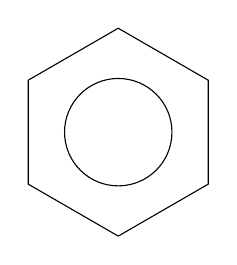
\begin{tikzpicture}[scale=1.1]
\draw (30:1.2) -- (90:1.2) -- (150:1.2) -- (210:1.2) -- (270:1.2) -- (330:1.2) -- cycle;
\draw (0,0) circle (0.62);
\end{tikzpicture}
\end{center}

This common drawing uses the hexagon for the six-carbon framework and circle for six delocalized electrons. It is a human-made symbol, not real lines or circles: the molecule has only electron clouds with varying probability distributions.

Electron laps have a measurable consequence: all six carbon--carbon bonds are identical. Ordinary single bonds measure about \ud{154}{pm}, doubles about \ud{134}{pm}; true alternation would alternate lengths. Measurements instead give six equal \ud{139}{pm} bonds, neatly between single and double. All carbons stand equal, no bond more single or double than another.

\section{Resonance: One Drawing Is Not Enough}

But our paper structures follow Chapter 17's convention, one line per bonding electron pair. Benzene's six delocalized electrons equal three double-bond pairs, yet none stays between a particular pair of carbons, and paper has no half-double-bond operation. Chemists therefore draw twice: one with a double bond between carbons 1 and 2, the other shifted to 2 and 3, joined by a double-headed arrow. Reality lies roughly between them. These are \textbf{resonance structures}, connected by a resonance arrow.

Here is the chapter's greatest trap and firm rule. Read twice: \textbf{benzene does not spend half its time as one drawing and half as the other, nor flip between them}. Throughout its existence, it has the same structure, six electrons distributed evenly over the whole ring. Neither individual drawing ever exists physically.

Think of a mule, offspring of horse and donkey. I can describe it as somewhat horse-like and somewhat donkey-like, but no mule is a horse half the time and donkey the other half, nor switches between them. Every second it is a mule. Horse and donkey are reference points for description. Likewise, resonance drawings are accounting tools, limited paper approximations of a structure one picture cannot capture. Understanding this gives you more insight than merely copying that benzene resonates.

Why insist on two drawings? One alternating-double-bond picture would assert unequal bond lengths and fixed electrons, contradicting measurements and stability. Two, plus other lesser contributors, can barely convey even electron distribution. Symbols accommodate reality, not the reverse.

\begin{qiaoliang}
How much energy does delocalization save? Try an imagined comparison. Cyclohexene has one double bond and releases about \ud{120}{kJ/mol} on hydrogenation to cyclohexane. If benzene had three independent ordinary doubles, hydrogenation should release $3\times 120=360$ \ud{}{kJ/mol}. Measurement gives only about \ud{208}{kJ/mol}, a difference near \ud{150}{kJ/mol}. Benzene lies that much below the hypothetical three-double-bond structure. This extra stability is \textbf{delocalization energy}, often aromatic stabilization energy, saved by the six electrons' laps. In Chapter 27's language, a lower-energy system is less inclined to change. Benzene resists easy alkene-like addition because it would dismantle the doughnut, first paying this \ud{150}{kJ/mol}, an unfavorable bargain.
\end{qiaoliang}

\section{Aromaticity: Stability Has Requirements}

Chemists call the unusually stable, cyclic, planar, ring-delocalized character \textbf{aromaticity}. Stability is always relative, Chapter 29 warned: benzene reacts selectively, not never. It prefers \textbf{substitution}, replacing one ring hydrogen with another atom or group while retaining the doughnut, rather than alkene-like addition that dismantles it. Alkenes readily add electron-poor reagents; benzene slowly accepts substitution with catalytic help.

Aromaticity is not benzene's monopoly. Life abounds in such rings: DNA bases, several amino-acid side chains, and key regions of light-sensitive molecules in your eyes contain aromatic rings or similar delocalized systems. Evolution repeatedly selected them over hundreds of millions of years for the same reasons chemists do: stable, flat, and conveniently sized components for molecular machines.

\section{Ring-Mounted Controls: Substituents and Electrons}

Benzene resembles a circular workbench whose character depends on attachments. These \textbf{substituents} redistribute ring electrons and add new reaction interfaces, directly continuing Chapter 37.

Some push electrons into the ring, such as hydroxyl, \chem{-OH}, and amino, \chem{-NH_2}, increasing electron richness and attraction for electron-poor reagents. Others pull electrons outward, such as nitro, \chem{-NO_2}, and carboxyl, \chem{-COOH}, thinning the ring's cloud and changing behavior.

Do not underestimate this push and pull. Compare familiar ethanol from Chapter 40 with phenol: both have hydroxyl, but aqueous ethanol is neutral and phenol distinctly weakly acidic. After hydrogen leaves a ring-mounted hydroxyl, the remaining negative charge spreads into the aromatic delocalized system, sharing the burden and easing release. The same hydroxyl on a chain gives alcohol, on an aromatic ring a weak acid. Structure determines electron distribution, which determines temperament: Chapter 32's causal thread returns.

Substituents also direct where newcomers attach. Pushers tend to guide them to neighboring ortho and opposite para positions; pullers prefer the alternative. Drug and dye synthesis uses these directing rules to plan order: attach the wrong group first, and misplaced impurities result. No mnemonic lies underneath, just electron-rich and electron-poor locations guiding reactions.

\section{Evidence: How the Hexagon Was Imaged}

\begin{zhengju}
Kekulé proposed benzene's hexagonal ring in 1865. Legend credits a dream of a snake biting its tail; its truth is uncertain. What is certain is that he never resolved why alternating single and double bonds failed to give alkene-like addition. For decades, competing prisms and centrally cross-linked structures persuaded nobody. Two independent sets of evidence eventually judged them.

First came crystals. In 1929, British crystallographer Kathleen Lonsdale used X-rays on hexamethylbenzene crystals. Regular atoms diffract X-rays, and spot positions reveal spatial arrangement, the method introduced in Chapter 24. The result was clear: six carbons in a flat regular hexagon, all carbon--carbon bonds equal. Prismatic candidates were eliminated.

Second came heat, the hydrogenation account already calculated: benzene releases about \ud{150}{kJ/mol} less than three ordinary doubles. Rapid switching between two structures alone cannot explain that lower energy; molecules do not save money merely by changing posture. Only one explanation fits both: electrons already spread over the ring, with wider distribution lowering energy. Later quantum calculations, extending Chapter 9's tools, reproduced bond lengths and energies precisely, closing the story.

Notice the chain: a useful but flawed structural hypothesis, two independent measurements eliminating alternatives, then theory explaining why. Not one genius's flash, but more than half a century of struggle.
\end{zhengju}
\section{Why Dyes Have Color}

Return to the jeans. The difference between white tablets and blue cloth lies in gaps between electron energy levels.

Chapter 9 placed electrons on energy floors; absorbing light matching a gap lets one jump. Benzene's delocalized electrons also have floors, but the gap is large, putting absorption in ultraviolet. Invisible ultraviolet leaves benzene colorless. Visible color requires shrinking the gap into the visible range.

The method is charmingly simple: \textbf{lengthen the delocalized track}. More spread-out electrons have closer levels and smaller gaps, moving absorption from ultraviolet toward visible. One benzene ring is insufficient, so link two through another delocalizing bridge, such as azo, \chem{-N=N-}. Azo dyes make up a major share of synthetic dyes today. Absorb one visible color range, and the remaining mixed light reaches your eyes as its \textbf{complement}: orange absorption looks blue, blue absorption yellow. Jeans' indigo is a long conjugated molecule absorbing orange-red light.

Substituents again serve as controls: hydroxyl or amino pushers on conjugated chains fine-tune gaps, changing shade and shifting redward or blueward. Dye engineers adjust colors by molecular structure.

For scale, visible photon energies are about $170$ to $300$ \ud{}{kJ/mol}, multiplying single-photon energy by Avogadro's constant. Benzene's delocalized transitions require more, in ultraviolet; each conjugated extension narrows the gap until it enters the $170$–$300$ window and color appears. The visible color world is essentially a map of molecular energy gaps.

An eighteen-year-old accidentally uncovered this principle in 1856. Perkin sought the antimalarial quinine from coal-tar materials, but a failed reaction left black sludge. Rather than discard it, he noticed a beautiful purple dissolved from it and dyed cloth brightly and durably. The first synthetic dye, mauveine, was born. Within decades, coal tar and aromatic rings supported a huge dye industry, freeing clothing colors from crushed plants and insects for the first time. Quinine was later synthesized too, but by a longer, more complicated story.

Color is not eternal. Strong light and oxygen attack conjugated dye chains; ultraviolet and atmospheric oxygen gradually sever them, enlarging gaps and fading fabric. That is why curtains whiten first on their outward-facing side.

\section{Medicines: An Aromatic Ring's Journey}

Now the tablet. Acetaminophen has a benzene ring with hydroxyl and amide opposite one another. After swallowing, it faces four stages whose outcomes are written in structure.

First, \textbf{dissolution}. A drug must dissolve in watery gastrointestinal fluid to be absorbed. Aromatic rings are oily: their hydrocarbon frameworks do not suit water, as Chapters 22 and 23's intermolecular forces explain, so purely aromatic compounds are mostly poorly soluble. Polar hydroxyl and amide form hydrogen bonds, built-in hydrophilic handles. Good drugs often balance oil and water affinity precisely: too hydrophilic to cross the next membrane barrier, too lipophilic to dissolve at all.

Second, \textbf{absorption and transport}. Cell membranes are oily barriers, detailed in Chapter 51, requiring some oil affinity for passage. Benzene's hydrocarbon segment supplies that passport.

Third, \textbf{binding}. A drug typically fits a protein-surface recess with complementary shape and charge, a key in a lock, explored in Chapters 48 and 49. Aromatic rings offer flat, rigid, fixed-size frameworks. Flexible chains twist, making a fit a matter of chance; a rigid ring is a defined key blank that firmly meets the right lock. Substituent positions shape its teeth.

Fourth, \textbf{metabolism}. The body treats foreign molecules as objects to process. Liver enzymes, protein catalysts obeying Chapters 30 and 49, punch holes in aromatic rings by adding hydroxyl and other polar groups, increasing water solubility for urinary elimination through the kidneys. Metabolic speed determines duration and \textbf{dose}. At ordinary acetaminophen doses, most is safely metabolized; excessive doses force a minor route into overdrive, producing a toxic intermediate that exhausts protective liver substances. This is the molecular basis of serious harm from common-drug overdose. Same molecule, different dose, different outcome. Enzyme activity, weight, and liver condition vary, so doses belong to physicians and instructions, never guesswork. We discuss principles only; follow medical advice for actual use.

Drug design---dissolution, absorption, binding, metabolism, dose---thus adds and subtracts structure: a ring for shape, hydroxyl for solubility, an exit for metabolism. Chapter 44's synthesis explores backward planning to build such molecules.

\section{Where Does This Model Fail?}

Time for honesty. Three tools came with boundaries: delocalized electrons, resonance notation, and structure-determines-properties reasoning.

Delocalization says wider spreading stabilizes electrons, but spreading requires geometry. Rings must be flat enough for adjacent orbital overlap. Some rings permit drawn alternating bonds yet twist out of plane, losing the benefit; without overlap, aromaticity is empty talk.

Resonance structures are accounts, not photographs. They help count electrons and estimate distribution, but asking which picture a molecule occupies now mistakes map for territory, the chapter's firm rule.

The greatest restraint is needed when predicting drug efficacy. Structure suggests solubility direction, candidate binding shapes, and metabolic sites, but an organism is a whole chemical city, revealed from Chapter 45 onward. Similar frameworks in different molecules or bodies can behave oppositely. Structure gives tendencies, not verdicts. New drugs need layers of experimental testing, not glorification based on drawings.

\begin{wuqu}
``Benzene rapidly switches between two structures, so measured bond lengths average out.'' This widespread misconception can even be encouraged by tautomerism. Two observations refute it. First, switching does not lower energy by \ud{150}{kJ/mol}, yet hydrogenation releases that much less; only electrons already spread out explain the savings. Second, switching predicts alkene behavior: even momentary double-bond forms should decolorize bromine water, but benzene refuses. Every moment benzene is its complete hybrid self. Our drawings switch, not the molecule.
\end{wuqu}

\begin{shiyan}
\textbf{Oil versus Water: Which Side Do Colors Choose?} (at home).

Materials: two clear glasses; clean water; a little cooking oil; food coloring or a drop of red or blue ink; a chopstick.

Procedure: (1) Half-fill each glass with water, add one coloring drop, stir, and record intensity. (2) Slowly pour about two spoonfuls of oil into one and wait for layers. (3) Stir gently and let settle, watching where the color goes. (4) Put a drop from each glass onto white paper and compare.

What to observe: most coloring molecules have polar groups, needed for water solubility, so almost all color stays in water and oil remains largely unstained. Polar handles determine destination, the same initial water-loving versus oil-loving choice in drug design.

Safety: food coloring is safe but stains persistently. Protect surfaces with newspaper and avoid pale clothes. Do not drink experimental liquids; wash hands afterward.
\end{shiyan}

\section{Back to the Tablet and Jeans}

Now fulfill the opening promise. The white tablet's benzene ring gives a flat rigid shape for protein locks; hydroxyl and amide are water-friendly handles and metabolic exits determining dissolution, duration, and safe dose. White results from absorption only in ultraviolet: its conjugation is too short to reach visible light.

Blue jeans have indigo's longer track, narrowing energy gaps into the visible window, absorbing orange-red and leaving blue. Descended directly from nineteenth-century coal-tar dyes, it too fades as sun and oxygen sever the track.

One hexagon, two uses: medicines use its \textbf{shape}, dyes its \textbf{electron energy levels}. One structural principle supports two industries, demonstrating recurring question two's power: how parts connect and arrange.

\section{Beyond the Plane: Left and Right Hands}

Our aromatic rings are flat. Almost every important bodily molecule, sugars, amino acids, drug targets, is three-dimensional, and many have a subtle left--right symmetry: mirror images that cannot overlap. Both hands share composition and connectivity but reverse spatial orientation. Life's precise machinery may treat them very differently: one heals, another is ineffective or harmful. Next chapter introduces these most subtle twins.

\begin{tiaozhan}
Which rings qualify as aromatic? In 1931, Hückel gave an electron-counting rule: a planar cyclic delocalized system is especially stable with $4n+2$ electrons, where $n$ is 0, 1, 2, and so forth. Benzene's six give $6=4\times 1+2$, aromatic. Cyclobutadiene's four give $4=4\times 1$, outside the favored list; it is extremely unstable and requires very low temperatures for observation. Naphthalene, an old mothball ingredient, shares ten electrons across two rings, $10=4\times 2+2$, also aromatic. Why these odd numbers? Quantum mechanics arranges ring-electron levels like seats, with $4n+2$ giving a closed shell of fully paired seats and no awkward half-fillings. Chapter 9's especially stable full atomic floors replay at molecular scale. You can skip this without losing the thread, but now you know what is special about six.
\end{tiaozhan}

\section*{Try It Yourself}

\begin{sikaoti}
\item Draw benzene's two alternating-double-bond resonance structures and the hexagon-with-circle version. For each, state what it expresses and what it cannot.
\item Cyclohexene adding one hydrogen molecule releases about \ud{120}{kJ/mol}. Predict the hydrogenation heat of hypothetical cyclohexatriene with three independent double bonds. Benzene actually gives about \ud{208}{kJ/mol}. Explain the energy difference and predict which more readily undergoes addition, benzene or cyclohexene.
\item Phenol's ring-mounted hydroxyl is weakly acidic; ethanol's chain-mounted hydroxyl is near neutral. Diagram the difference using whether negative charge can spread into a delocalized system.
\item A yellow dye absorbs blue light. Add another benzene ring to extend its conjugated track: does absorption shift to longer or shorter wavelengths, and how might color shift?
\item A highly oily drug dissolves poorly and has poor oral absorption. A pharmacist introduces a negatively charged polar group to make a salt. Analyze benefits and possible costs at the dissolution and membrane-crossing stages.
\item A student says benzene spends equal time in two resonance forms, making average bond lengths. Refute this with the two experimental facts and state the correct interpretation.
\end{sikaoti}
